\documentclass[10pt, a4paper, notitlepage]{article}
\usepackage{tikz}
\usetikzlibrary{calc}
\usetikzlibrary{cd}
\usetikzlibrary{decorations.markings}
\usetikzlibrary{decorations.pathreplacing}
\usetikzlibrary{decorations.pathmorphing}
\usetikzlibrary{decorations.text}
\usetikzlibrary{arrows.meta}
\usetikzlibrary{arrows}
\usetikzlibrary{positioning}
\usepackage{amssymb}
\usepackage{amsmath}

\newcommand{\smooth}[1]{\tilde{#1}}

\begin{document}

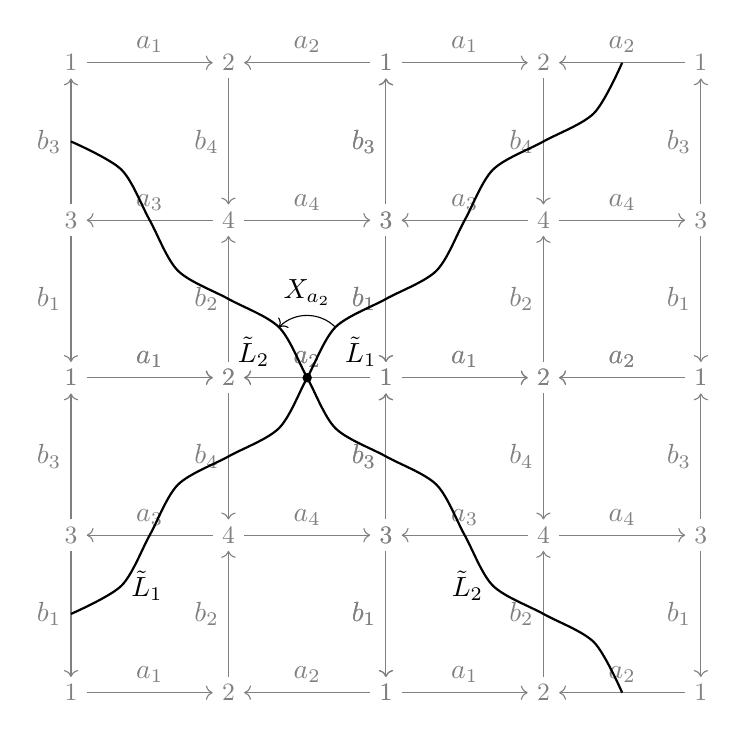
\begin{tikzpicture}[scale=2]
\newcommand{\arrowbetween}[2]{($ (#1)!0.1!(#2) $) -- ($ (#2)!0.1!(#1) $)}
\newcommand{\thetorus}{%
% horizontal
\path[draw, ->] \arrowbetween{0, 0}{1, 0} node[midway, above] {$ a_1 $};
\path[draw, ->] \arrowbetween{2, 0}{1, 0} node[midway, above] {$ a_2 $};
\path[draw, ->] \arrowbetween{0, 2}{1, 2} node[midway, above] {$ a_1 $};
\path[draw, ->] \arrowbetween{2, 2}{1, 2} node[midway, above] {$ a_2 $};
\path[draw, ->] \arrowbetween{1, 1}{0, 1} node[midway, above] {$ a_3 $};
\path[draw, ->] \arrowbetween{1, 1}{2, 1} node[midway, above] {$ a_4 $};
%
\path[draw, ->] \arrowbetween{0, 1}{0, 0} node[midway, left] {$ b_1 $};
\path[draw, ->] \arrowbetween{0, 1}{0, 2} node[midway, left] {$ b_3 $};
\path[draw, ->] \arrowbetween{2, 1}{2, 0} node[midway, left] {$ b_1 $};
\path[draw, ->] \arrowbetween{2, 1}{2, 2} node[midway, left] {$ b_3 $};
\path[draw, ->] \arrowbetween{1, 0}{1, 1} node[midway, left] {$ b_2 $};
\path[draw, ->] \arrowbetween{1, 2}{1, 1} node[midway, left] {$ b_4 $};
%
\path (0, 0) node {\small $ 1 $};
\path (2, 0) node {\small $ 1 $};
\path (2, 2) node {\small $ 1 $};
\path (0, 2) node {\small $ 1 $};
\path (1, 0) node {\small $ 2 $};
\path (1, 2) node {\small $ 2 $};
\path (0, 1) node {\small $ 3 $};
\path (2, 1) node {\small $ 3 $};
\path (1, 1) node {\small $ 4 $};}
%
\begin{scope}[shift={(2, 0)}, every path/.style={gray}] \thetorus \end{scope}
\begin{scope}[shift={(2, 2)}, every path/.style={gray}] \thetorus \end{scope}
\begin{scope}[shift={(4, 0)}, every path/.style={gray}] \thetorus \end{scope}
\begin{scope}[shift={(4, 2)}, every path/.style={gray}] \thetorus \end{scope}
%
\path[draw, thick] plot[smooth] coordinates{(2, 0.5) ($ (2.25, 0.75) + (315:0.1) $) (2.5, 1) ($ (2.75, 1.25) + (135:0.1) $) (3, 1.5) ($ (3.25, 1.75) + (315:0.1) $) (3.5, 2) ($ (3.75, 2.25) + (135:0.1) $) (4, 2.5) ($ (4.25, 2.75) + (315:0.1) $) (4.5, 3) ($ (4.75, 3.25) + (135:0.1) $) (5, 3.5) ($ (5.25, 3.75) + (315:0.1) $) (5.5, 4)};
\path[draw, thick] plot[smooth] coordinates{(5.5, 0) ($ (5.25, 0.25) + (45:0.1) $) (5, 0.5) ($ (4.75, 0.75) + (225:0.1) $) (4.5, 1) ($ (4.25, 1.25) + (45:0.1) $) (4, 1.5) ($ (3.75, 1.75) + (225:0.1) $) (3.5, 2) ($ (3.25, 2.25) + (45:0.1) $) (3, 2.5) ($ (2.75, 2.75) + (225:0.1) $) (2.5, 3) ($ (2.25, 3.25) + (45:0.1) $) (2, 3.5)};
\path[fill] (3.5, 2) circle[radius=0.03];
\path[draw, bend right=45, ->] ($ (3.75, 2.25) + (135:0.1) $) to node[above] {$ X_{a_2} $} node[at start, below right] {$ \smooth L_1 $} node[at end, below left] {$ \smooth L_2 $} ($ (3.25, 2.25) + (45:0.1) $);
\path ($ (4.75, 0.75) + (225:0.1) $) node[left] {$ \smooth L_2 $};
\path ($ (2.25, 0.75) + (315:0.1) $) node[right] {$ \smooth L_1 $};
\end{tikzpicture}

\end{document}